\documentclass[11pt]{article}
\usepackage[margin=1.1in]{geometry}
\usepackage{booktabs, graphicx, amsmath, amssymb}
\usepackage[labelfont=bf]{caption}
\usepackage{setspace}
\usepackage[dvipsnames]{xcolor}
\usepackage[colorlinks=true, allcolors=BrickRed]{hyperref}
\usepackage{titlesec}
\titleformat{\section}{\large\bfseries}{\thesection.}{0.6em}{}
\titleformat{\subsection}{\normalsize\bfseries}{\thesubsection.}{0.6em}{}

% All numbers below are generated by code/memo/01_memo_stats.R.
% Nothing in this document is typed by hand.
\newcommand{\polNatlApr}{0.42}
\newcommand{\polNatlMay}{0.46}
\newcommand{\elecNatlApr}{0.04}
\newcommand{\elecNatlMay}{0.07}
\newcommand{\newsNatlMay}{0.49}
\newcommand{\polOneInN}{217}
\newcommand{\nCountries}{59}
\newcommand{\ctyTopName}{USA}
\newcommand{\ctyTopVal}{0.46}
\newcommand{\ctyBotName}{VNM}
\newcommand{\ctyBotVal}{0.09}
\newcommand{\ctyRatio}{5.1}
\newcommand{\usaRank}{1}
\newcommand{\usePersonal}{78.4}
\newcommand{\useWork}{18.9}
\newcommand{\useCoursework}{2.7}
\newcommand{\collabAutomation}{41.7}
\newcommand{\collabAugmentation}{58.3}
\newcommand{\artInfoShare}{67.6}
\newcommand{\artDoingShare}{2.8}
\newcommand{\artInfoDoingRatio}{24}
\newcommand{\artExplain}{47.7}
\newcommand{\artExplainAll}{16.7}
\newcommand{\artAnalysis}{19.9}
\newcommand{\artEmail}{0.9}
\newcommand{\artEmailAll}{4.6}
\newcommand{\artPlan}{1.8}
\newcommand{\artNone}{15.0}
\newcommand{\patLearning}{40.7}
\newcommand{\gfInfo}{28.2}
\newcommand{\gfAction}{11.1}
\newcommand{\gfDoc}{39.6}
\newcommand{\gfShare}{0.06}
\newcommand{\elInfo}{62.4}
\newcommand{\elAction}{1.2}
\newcommand{\prInfo}{64.9}
\newcommand{\prAction}{0.2}
\newcommand{\polTopicInfo}{74.4}
\newcommand{\nDetailed}{1012}
\newcommand{\nMinor}{196}
\newcommand{\nMajor}{20}
\newcommand{\mainEst}{0.10}
\newcommand{\mainSE}{0.04}
\newcommand{\mainT}{2.61}
\newcommand{\mainBase}{0.48}
\newcommand{\mainPct}{22}
\newcommand{\mainStates}{30}
\newcommand{\mainTreated}{8}
\newcommand{\logEst}{0.24}
\newcommand{\logSE}{0.09}
\newcommand{\noJuneEst}{0.09}
\newcommand{\noJuneSE}{0.04}
\newcommand{\nullN}{210}
\newcommand{\polRank}{3}
\newcommand{\riP}{0.024}
\newcommand{\nullSD}{1.17}
\newcommand{\nullMean}{-0.03}
\newcommand{\nSig}{21}
\newcommand{\pctSig}{10}
\newcommand{\nAbove}{3}
\newcommand{\nMayPrimary}{11}
\newcommand{\nMayKept}{8}
\newcommand{\nMayDropped}{3}
\newcommand{\mayDroppedList}{KY, NE, WV}

\graphicspath{{../../output/memo/}}

\title{\textbf{Political Conversations with Claude}\\[2mm]
\large How Much, Where, and Whether Elections Move Them}
\author{Andrew B. Hall \and Daniel M. Thompson}
\date{\today}

\begin{document}
\maketitle
\onehalfspacing

\begin{abstract}
\noindent Using the Anthropic Economic Index's public state-month topic shares, we document
how much of Claude usage is political, what people are doing when they raise
politics, and whether elections move it. Politics is a small share of all
conversations---\polNatlMay\% in May 2026, or roughly one conversation in
\polOneInN---and is overwhelmingly personal rather than work-related. It is also
overwhelmingly \emph{informational}: \artInfoShare\% of political conversations
produce an explanation or an analysis, while only \artDoingShare\% produce a
message, a plan, or organizing content---a ratio of about
\artInfoDoingRatio\ to 1. People are using Claude to understand politics, not yet
to act in it. We then ask whether holding a primary election moves the political
share. States with May 2026 primaries saw a \mainEst\ percentage-point increase
off a \mainBase\% base, about \mainPct\%. The effect is specific: it appears for
politics and not for news, geopolitics, or a non-political comparison topic.
Applying the identical specification to all \nullN\ topics in the release,
politics ranks \polRank rd largest, giving a randomization-inference $p$-value of
\riP.
\end{abstract}

\section{Data}

All figures come from the Anthropic Economic Index (AEI) release of 26 June 2026
(CC-BY, \href{https://huggingface.co/datasets/Anthropic/EconomicIndex}{Hugging Face}),
which reports the share of Claude conversations assigned to each request topic for
April and May 2026, at global, country, and US state level. Two features of the data
govern everything that follows. First, shares are rounded to two decimals, so the
measurement grid is coarse relative to the effects at issue. Second, a missing
state-topic cell means the cell fell below Anthropic's privacy threshold, not that
the share was zero. Topic taxonomies are re-clustered in every release, so these
shares are not comparable to earlier or later AEI releases.

Primary dates are hand-compiled from NCSL and FVAP, which agree; the file and its
sources are documented in \texttt{original\_data/primary\_dates/}.

\subsection{How Anthropic codes conversations}

Because everything below depends on it, it is worth being precise about how these
categories are produced. All AEI classification is done by
\href{https://www.anthropic.com/research/clio}{Clio}, Anthropic's
privacy-preserving analysis system: conversation transcripts are read only by
another instance of Claude, never by a human, and cells with too few
observations are suppressed before release. Every variable we use is therefore a
model-assigned label aggregated over sampled conversations, not a human-coded one.

\textbf{The topic hierarchy.} Requests are grouped into a three-level topic
tree. Level 0 (``Detailed'') has \nDetailed\ topics, level 1 (``Minor'') has
\nMinor, and level 2 (``Major'') has \nMajor. Our outcome, ``Politics and public
record,'' is a \emph{Minor} topic, while ``Politics'' and ``Elections'' are
Detailed topics. The published file gives each node's level but not its parent,
so while the levels are ordered by aggregation we cannot confirm from the data
which Detailed topics roll up into which Minor one. Critically, this taxonomy is re-clustered from scratch in every
release, so a topic's share cannot be compared across releases even under the
same name.

\textbf{Use case} assigns each conversation to \texttt{work}, \texttt{personal},
or \texttt{coursework}.

\textbf{Collaboration pattern} assigns each conversation to one of five modes
(defined in Panel C of Table~\ref{tab:composition}). These are then collapsed
into two buckets: \emph{automation} (directive or feedback loop) and
\emph{augmentation} (task iteration, learning, or validation). One subtlety
matters for reading the numbers: the buckets renormalize over conversations that
received a pattern, excluding the \texttt{none} category, so bucket shares sum
to 100 while pattern shares sum to 100 only once \texttt{none} is included. We
verified this against the data---directive plus feedback loop, divided by one
minus the \texttt{none} share, reproduces the published automation figure
exactly---and the check is asserted in the code that generates this memo.

\textbf{Artifact} records the single most prominent concrete output the
conversation produced, across \mbox{30-odd} labels plus \texttt{none}. This is
the variable we lean on hardest below, because it distinguishes a conversation
that ended in an explanation from one that ended in a draft email.

\textbf{A note on reading the tables.} Because these classifications are
nested in some places and merely parallel in others, every table below that
mixes them is split into labelled panels. Rows within a panel are mutually
comparable and, where noted, sum to 100. Rows in different panels are
\emph{not} comparable and must never be added together. In particular, AEI does
not publish the parent-child map linking Detailed topics to their Minor
parents, so we never assert that a given Detailed topic sits beneath a given
Minor one.

\section{Descriptives}

\subsection{Politics is a small share of conversations}

In May 2026, \polNatlMay\% of US Claude conversations were assigned to
``Politics and public record,'' up from \polNatlApr\% in April. That is
roughly one conversation in \polOneInN. The narrower ``Elections'' topic is
smaller still, at \elecNatlMay\% in May. Any claim about AI and political
information should be read against this base: political conversation is a
rounding error in aggregate Claude usage, before and after any election.

Table~\ref{tab:topics} decomposes the political topics, split by taxonomy level.
Panel A holds the Minor topics---aggregates, one of which is our outcome---and
Panel B the Detailed leaves. Keeping them apart matters: ``News aggregation''
(\newsNatlMay\% in May) is numerically larger than ``Politics and public
record'' (\polNatlMay\%), but it is a Detailed topic and the latter is a Minor
one, so the comparison is between units at different levels of aggregation
rather than between a category and its sub-category. The rightmost columns show
how few states clear the privacy threshold for the narrower topics, which is why
the analysis below uses the broad politics measure as its outcome.

\begin{table}[h!]
\centering
\caption{Political and News Topics: National Shares and State Coverage\label{tab:topics}}
\begin{tabular}{lcccc}
\toprule \toprule
 & \multicolumn{2}{c}{US National Share (\%)} & \multicolumn{2}{c}{\# States Reported} \\
\cmidrule(lr){2-3} \cmidrule(lr){4-5}
 & April & May & April & May \\
\midrule
\addlinespace
\multicolumn{5}{l}{\textit{Panel A. Minor topics (level 1, aggregates)}} \\[0.5mm]
\quad Politics and public record & 0.42 & 0.46 & 36 & 35 \\
\quad Geopolitics and strategy & 0.20 & 0.15 & 21 & 22 \\
\quad Government filings & 0.06 & 0.06 & 7 & 7 \\
\addlinespace
\multicolumn{5}{l}{\textit{Panel B. Detailed topics (level 0, leaves)}} \\[0.5mm]
\quad News aggregation & 0.42 & 0.49 & 29 & 34 \\
\quad News writing & 0.15 & 0.16 & 20 & 24 \\
\quad Politics & 0.14 & 0.15 & 19 & 25 \\
\quad Geopolitics & 0.08 & 0.07 & 7 & 11 \\
\quad Elections & 0.04 & 0.07 & 3 & 8 \\
\quad Public records lookup & 0.05 & 0.05 & 4 & 12 \\
\bottomrule \bottomrule
\end{tabular}

\end{table}

\begin{figure}[h!]
\centering
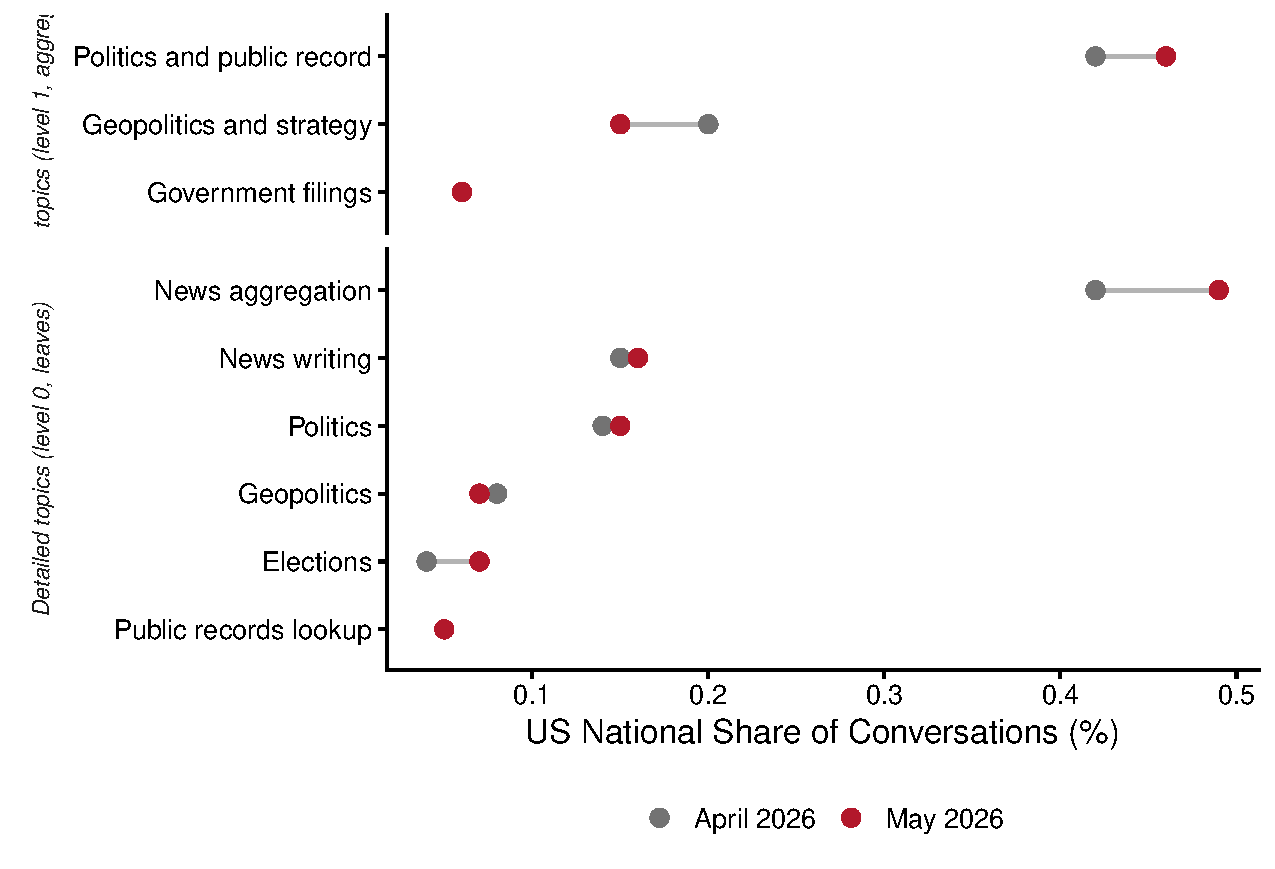
\includegraphics[width=0.78\textwidth]{fig_topic_decomposition.pdf}
\caption{\textbf{What kinds of politics people bring to Claude.} US national
shares of all Claude conversations, May 2026, by request topic. The two panels
are separate levels of the AEI taxonomy and overlap in coverage, so they should
not be added together. News-seeking dominates: ``News aggregation''
(\newsNatlMay\%) is larger than any other topic shown, while explicitly
electoral use (``Elections,'' \elecNatlMay\%) is far
smaller.\label{fig:topics}}
\end{figure}

\subsection{The United States is the most political market}

Across the \nCountries\ countries for which the politics share is reported in May
2026, the United States ranks \usaRank st at \ctyTopVal\%, against
\ctyBotVal\% at the bottom (\ctyBotName)---a spread of roughly
\ctyRatio$\times$ (Figure~\ref{fig:country}). Political use of Claude is not
uniform across markets, and the US sits at the top of the distribution rather
than in the middle of it.

\begin{figure}[h!]
\centering
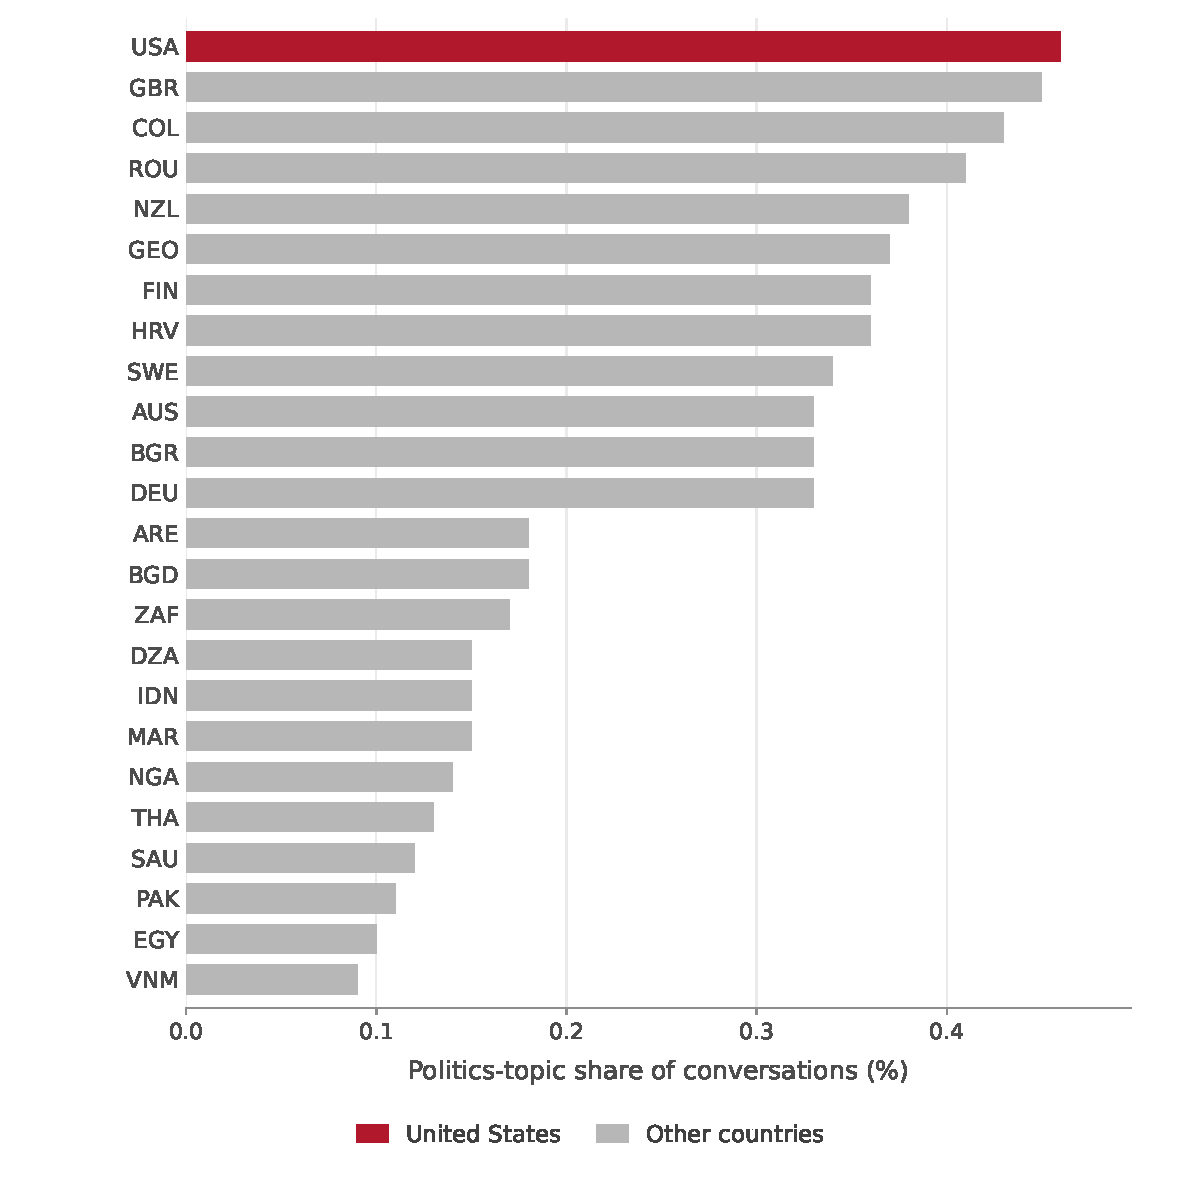
\includegraphics[width=0.62\textwidth]{fig_country_shares.pdf}
\caption{\textbf{Politics-topic share by country, May 2026.} Twelve highest and
twelve lowest of \nCountries\ reported countries.\label{fig:country}}
\end{figure}

\subsection{Political use is personal, not professional}

Table~\ref{tab:composition} reports how political conversations are conducted.
The pattern is stark: \usePersonal\% of politics conversations are personal
use, against only \useWork\% work use and \useCoursework\% coursework. Whatever
people are doing when they ask Claude about politics, they are mostly not doing
their jobs. Interaction style is majority augmentation (\collabAugmentation\%)
rather than automation (\collabAutomation\%), and both shift slightly toward
augmentation between April and May.

\begin{table}[h!]
\centering
\caption{How Political Conversations Are Conducted (Global, \%)\label{tab:composition}}
\begin{tabular}{llccc}
\toprule \toprule
 & Definition & April & May & Change \\
\midrule
\addlinespace
\multicolumn{5}{l}{\textit{Panel A. Use case (sums to 100)}} \\[0.5mm]
\quad Personal & & 77.7 & 78.4 & 0.7 \\
\quad Work & & 19.7 & 18.9 & -0.8 \\
\quad Coursework & & 2.6 & 2.7 & 0.1 \\
\addlinespace
\multicolumn{5}{l}{\textit{Panel B. Collaboration bucket (sums to 100, excludes \textit{none})}} \\[0.5mm]
\quad Augmentation & Task iteration, learning, or validation & 56.9 & 58.3 & 1.4 \\
\quad Automation & Directive or feedback loop & 43.1 & 41.7 & -1.4 \\
\addlinespace
\multicolumn{5}{l}{\textit{Panel C. Collaboration pattern (sums to 100; Panel B is built from these)}} \\[0.5mm]
\quad Learning & Seeking understanding & 40.5 & 40.7 & 0.2 \\
\quad Directive & Minimal human interaction & 35.0 & 33.9 & -1.1 \\
\quad Task iteration & Human refines AI outputs & 12.0 & 13.3 & 1.2 \\
\quad Feedback loop & Iterative dialogue with feedback & 6.9 & 6.7 & -0.2 \\
\quad Validation & Human checking own work & 2.9 & 2.9 & -0.0 \\
\quad None & No pattern assigned & 2.7 & 2.6 & -0.1 \\
\bottomrule \bottomrule
\end{tabular}

\end{table}

\noindent A caveat that constrains this section: these behavioral metrics are
published \emph{only} at the global level. Country and state cells carry the
topic share alone. The composition results are therefore descriptive and cannot
be linked to the state-level variation used below.

\subsection{Seeking information about politics versus doing politics}
\label{sec:info-doing}

The composition numbers hint at something the artifact data make unmistakable.
Table~\ref{tab:artifacts} and Figure~\ref{fig:artifacts} compare what political
conversations produce against the baseline across all Claude conversations.

Political conversations are dominated by outputs that transmit understanding.
\artExplain\% end in an explanation or answer, against \artExplainAll\% of
conversations generally---nearly three times the rate. Another \artAnalysis\%
end in an analysis or summary. Together, \artInfoShare\% of political
conversations produce an explanation or an analysis.

Outputs that constitute political \emph{action} are not merely rare in absolute
terms; they are rarer than in ordinary Claude usage. Only \artEmail\% of
political conversations produce an email or message---the artifact one would
expect from contacting a representative, writing public comment, or organizing---
against \artEmailAll\% of conversations generally. Plans or strategies account
for \artPlan\%. Summing the action-shaped artifacts gives \artDoingShare\%,
against \artInfoShare\% for the information-shaped ones: a ratio of roughly
\artInfoDoingRatio\ to 1. The collaboration patterns tell the same story from a
different angle, with \patLearning\% of political conversations classified as
\emph{learning}---seeking understanding---the single largest pattern
(Table~\ref{tab:composition}, Panel C).

\begin{table}[h!]
\centering
\caption{Artifacts Most Over- and Under-Represented in Political Conversations
(Global, May 2026)\label{tab:artifacts}}
\begin{tabular}{lccc}
\toprule \toprule
Artifact produced & Politics (\%) & All conversations (\%) & Difference \\
\midrule
Explanation or answer & 47.7 & 16.7 & 31.1 \\
Analysis or summary & 19.9 & 5.5 & 14.3 \\
None & 15.0 & 6.5 & 8.5 \\
Script or snippet & 0.2 & 3.0 & -2.8 \\
Educational material & 0.0 & 2.8 & -2.8 \\
Code fix or debug & 0.0 & 3.3 & -3.3 \\
Email or message & 0.9 & 4.6 & -3.7 \\
App or website & 0.3 & 4.2 & -3.9 \\
Advice or recommendation & 3.3 & 10.7 & -7.4 \\
Document or report & 6.6 & 14.9 & -8.3 \\
\bottomrule \bottomrule
\end{tabular}

\end{table}

\begin{figure}[h!]
\centering
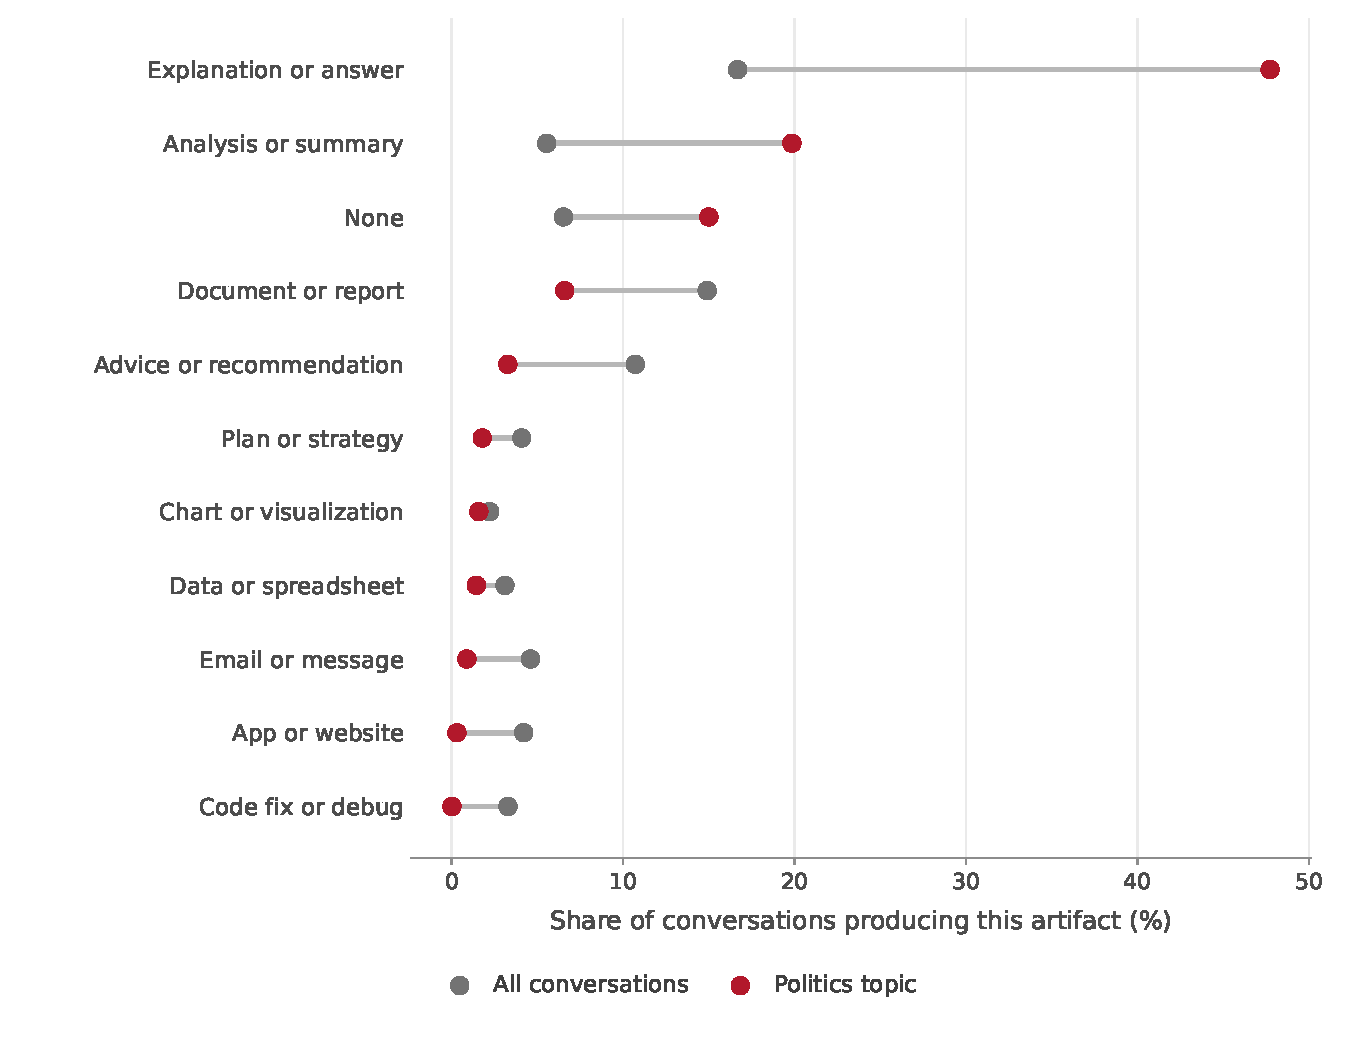
\includegraphics[width=0.85\textwidth]{fig_artifacts.pdf}
\caption{\textbf{What political conversations produce.} Share of conversations
whose most prominent output is each artifact type, politics topic versus all
conversations.\label{fig:artifacts}}
\end{figure}

\subsection{Reading this through the three layers}

Hall's framework for AI and democracy distinguishes three layers at which the
technology could matter: an \emph{information} layer, in which AI makes citizens
and governments smarter; a \emph{representation} layer, in which AI acts on
citizens' behalf so that their interests are conveyed faithfully; and a
\emph{governance} layer, in which we set the rules under which the AI systems
themselves operate.\footnote{Andrew B. Hall, ``Building Political
Superintelligence,'' \emph{Free Systems}, March 26, 2026.} The
artifact distribution offers the first direct measurement we are aware of how
present-day usage divides across them.

The headline is that the information layer dominates---but the aggregate hides
a distinction that matters for the framework, and Table~\ref{tab:profile} draws
it out by running the same artifact split topic by topic.

\begin{table}[h!]
\centering
\caption{Information, Action, and Document Artifacts by Topic (Global, May 2026)\label{tab:profile}}
\begin{tabular}{llcccc}
\toprule \toprule
Topic & Level & Share (\%) & Information & Action & Document \\
\midrule
Politics & Detailed & 0.15 & 74.4 & 1.1 & 3.3 \\
Politics and public record & Minor & 0.46 & 67.6 & 2.8 & 8.1 \\
Public records lookup & Detailed & 0.05 & 64.9 & 0.2 & 4.0 \\
Elections & Detailed & 0.07 & 62.4 & 1.2 & 6.2 \\
Government filings & Minor & 0.06 & 28.2 & 11.1 & 39.6 \\
\bottomrule \bottomrule
\end{tabular}

\end{table}

\textbf{The civic-informational topics are overwhelmingly informational.}
``Politics'' is \polTopicInfo\% explanation-or-analysis, ``Elections''
\elInfo\%, and---despite its transactional-sounding name---``Public records
lookup'' \prInfo\%. Action artifacts are near zero across all three
(\elAction\% for Elections, \prAction\% for public records). A public-records
lookup turns out to be exactly what it says: a lookup. This is Condorcet's
printing-press argument running on new hardware, and the primary-election
result in Section~\ref{sec:did} shows it responding to the electoral calendar
exactly as a demand-for-information story predicts.

\textbf{``Government filings'' is the exception, and it is a different kind of
thing entirely.} Only \gfInfo\% of those conversations produce an explanation or
analysis. Instead \gfDoc\% produce a document or report and \gfAction\% produce
action artifacts---four times the action rate of any civic topic. Here people
genuinely are using Claude to \emph{do} something with government rather than to
learn about it.

This is what resolves the puzzle that government filings and public records
appear at magnitudes comparable to elections. Two different things are going on.
Some of it is an artifact of the taxonomy: ``Government filings'' is a Minor
topic (\gfShare\%) and ``Elections'' a Detailed one, so their raw shares were
never like-for-like. But the substantive point survives the correction:
administrative engagement with government is real, is roughly the scale of
electoral interest, and---unlike electoral interest---involves actual production.

Crucially, that production is not \emph{representation}. Filing a form, claiming
a benefit, or navigating an agency is the citizen acting as a client of the
state, not as a principal directing an agent. In Hall's terms it belongs to the
service-delivery strand of the information layer---government working better for
the people who deal with it---rather than to the representation layer, which
concerns whether citizens' interests are conveyed faithfully into political
decisions. Nothing in these data looks like drafting comments to agencies,
contacting legislators, or coordinating with neighbors. The representation layer
remains close to empty even in the one topic where people are visibly doing
things.

The governance layer is, unsurprisingly, invisible here, and would be even if it
were thriving: deliberation over the rules governing AI systems is not something
one would expect to observe in the topic distribution of consumer chat.

\textbf{The takeaway.} Present-day political usage of Claude is concentrated in
the information layer, and splits within it into a large civic-informational
strand (learning about politics and elections) and a smaller administrative
strand (transacting with government) that is the only place action-shaped output
appears at all. The representation layer, where AI would act on citizens'
behalf, is not yet visible in consumer usage. If the information layer is where
the technology is arriving first, that is where its near-term democratic
effects---good and bad---will be concentrated.

Two cautions before this is read as a verdict. First, the AEI covers Claude's
consumer surfaces; agentic and API traffic, where representation-layer activity
would more plausibly live, is either excluded or reported only globally.
Second, an artifact label captures the most prominent output of a conversation,
so a conversation that informed someone who later acted is coded as information.
What we can say is narrower than ``AI is not being used for political action'':
it is that within consumer Claude usage, informational political activity
currently outweighs action-shaped political activity by more than an order of
magnitude. If the information layer is where the technology is currently
arriving, that is where its near-term democratic effects---good and bad---will be
concentrated.

\section{Do Primaries Move Political Conversation?}
\label{sec:did}

\subsection{Design}

We compare states holding a statewide primary in May 2026 to states with later
primaries, before and after. For state $s$ in month $t$,
%
\begin{equation}
y_{st} = \beta \,(\text{Primary}_s \times \text{May}_t) + \alpha_s + \delta_t + \varepsilon_{st},
\end{equation}
%
where $y_{st}$ is the politics-topic share, $\alpha_s$ and $\delta_t$ are state
and month fixed effects, and standard errors are clustered by state. The panel is
balanced across April and May. States holding March primaries (TX, NC, IL) are
already treated and are dropped throughout. The estimation sample is
\mainStates\ states, \mainTreated\ of them treated.

\subsection{Main result}

\begin{table}[t]
\centering
\caption{\textbf{Claude Conversations Shift Toward Politics When a State Holds Its Primary.}\label{tab:aei_did}}
\begin{tabular}{lccc}
\toprule \toprule
 & \multicolumn{2}{c}{Politics-Topic Share (\%)} & Log Share \\
\cmidrule(lr){2-3} \cmidrule(lr){4-4}
 & (1) & (2) & (3) \\
\midrule
Primary $\times$ May & 0.10 & 0.09 & 0.24 \\
 & (0.04) & (0.04) & (0.09) \\[2mm]
\# States & 30 & 20 & 30 \\
\# Treated States & 8 & 8 & 8 \\
\# Observations & 60 & 40 & 60 \\
Control May Mean & 0.48 & 0.45 & 0.48 \\
Minimum Detectable Effect & 0.11 & 0.12 & 0.24 \\
\midrule
State Fixed Effects & Yes & Yes & Yes \\
Month Fixed Effects & Yes & Yes & Yes \\
Excl.\ June-Primary Controls & No & Yes & No \\
\bottomrule \bottomrule
\multicolumn{4}{p{0.95\textwidth}}{\footnotesize \textit{Notes}: Each column reports a difference-in-differences estimate comparing the politics-topic share of Claude conversations in April and May 2026 between states holding a statewide primary in May 2026 and states with later primaries. The outcome in columns 1 and 2 is the percent of a state's conversations assigned to the ``Politics and public record'' topic in the Anthropic Economic Index; column 3 uses its natural log. Texas, North Carolina, and Illinois, which held March primaries, are excluded. Column 2 further drops control states with June primaries, whose mail voting begins in May. Standard errors clustered by state are in parentheses. The minimum detectable effect is 2.80 times the standard error.} \\
\end{tabular}
\end{table}


\noindent Holding a May primary raises the politics share by \mainEst\ percentage
points (s.e.\ \mainSE, $t=\mainT$) on a control-group base of \mainBase\%---an
increase of about \mainPct\%. In levels this moves a state from roughly one
political conversation in 250 to one in 200.

\subsection{The effect is specific to politics}

If the estimate reflected a general election-season rise in information seeking,
it should appear in adjacent topics too. It does not. Table~\ref{tab:spec}
applies the identical specification to news aggregation, news writing,
geopolitics, and a non-political comparison topic. All four are small and
statistically indistinguishable from zero, and their standard errors are if
anything tighter than the main estimate's---so they are precise enough to have
detected an effect the size of the politics result had one been present.
Domestic politics moves; foreign affairs and general news do not.

\begin{table}[h!]
\centering
\caption{Specificity: The Same Design Applied to Adjacent Topics\label{tab:spec}}
\begin{tabular}{lccccc}
\toprule \toprule
Topic & Estimate & (SE) & $t$ & \# States & \# Treated \\
\midrule
\textbf{Politics and public record} & 0.10 & (0.04) & 2.61 & 30 & 8 \\
Geopolitics and strategy & -0.01 & (0.02) & -0.39 & 16 & 4 \\
Personal finance & -0.01 & (0.03) & -0.44 & 25 & 6 \\
News writing & -0.02 & (0.03) & -0.55 & 16 & 4 \\
News aggregation & -0.04 & (0.03) & -1.17 & 26 & 6 \\
\bottomrule \bottomrule
\end{tabular}

\end{table}

\subsection{A permutation test across all topics}

The sharpest test available is to apply the identical design to every topic in
the release and ask how unusual the politics estimate is. Among the \nullN\
topic series with sufficient state coverage, politics ranks \polRank rd by
$t$-statistic, and \nAbove\ topics have a $t$ at least as large in absolute
value. That yields a randomization-inference $p$-value of \riP\ without
relying on the clustered standard errors at all (Figure~\ref{fig:null}).

\begin{figure}[h!]
\centering
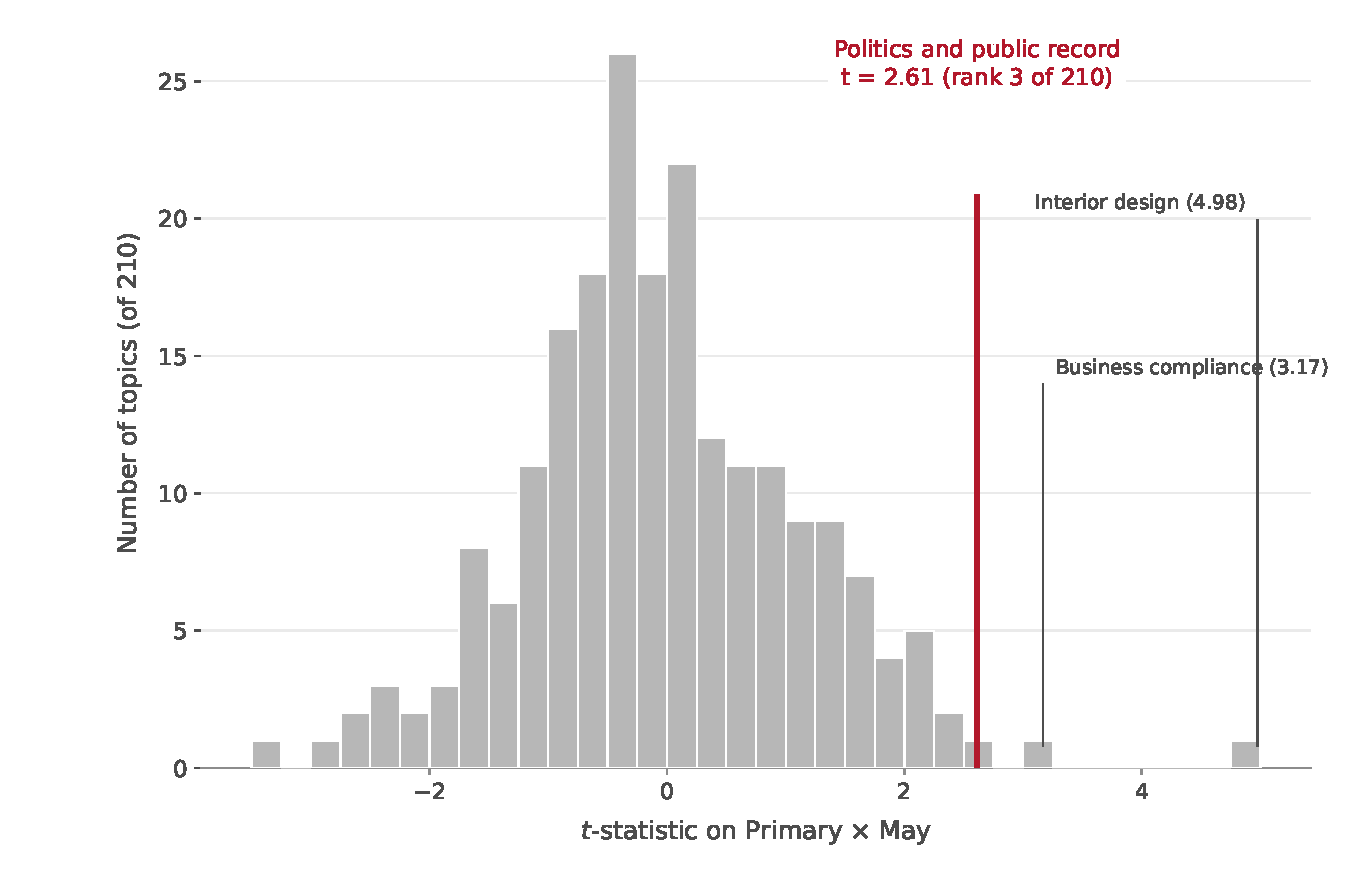
\includegraphics[width=0.85\textwidth]{fig_null_distribution.pdf}
\caption{\textbf{Empirical null distribution.} Distribution of $t$-statistics on
Primary $\times$ May across all \nullN\ topic series estimable with the same
specification.\label{fig:null}}
\end{figure}

\noindent Two features of this distribution deserve comment. It is centered
essentially at zero (mean \nullMean), which is reassuring: the design is not
mechanically manufacturing effects. But its dispersion exceeds the nominal
(s.d.\ \nullSD\ against 1.00 under correctly sized standard errors), and
\nSig\ of \nullN\ topics---\pctSig\%---clear $|t| \geq 1.96$ against the 5\%
expected by chance. Conventional standard errors are therefore modestly too
small here, which is exactly why the permutation $p$-value is the number to
report. Some unrelated topics do land above politics; with \nullN\ tests that
is expected, and the permutation test prices it in rather than being
embarrassed by it.

\section{Limitations}

\textbf{Two periods, so no pre-trends.} With only April and May, parallel trends
is assumed rather than tested. A third month would allow a genuine pre-trend
check and is the single most valuable addition a future AEI release could make.

\textbf{Treated states are lost to the balance requirement.} Of \nMayPrimary\
May-primary states, \nMayKept\ survive into the estimation sample; \nMayDropped\
(\mayDroppedList) are dropped because they fall below the privacy threshold in
at least one month. These are small states, so this is most likely a volume
artifact, but the treatment group is \nMayDropped/\nMayPrimary\ smaller than the
calendar implies.

\textbf{Coarse measurement.} Shares are rounded to two decimals, so the effect
is ten rounding increments wide.

\textbf{No comparable data elsewhere.} Replicating this design with Google or
OpenAI data is currently impossible. Google's AI \& Economy ATLAS (July 2026)
reports country-level data for a single two-week window and publishes no
dataset. OpenAI Signals publishes monthly state data under CC-BY, but its topic
taxonomy is functional (programming, cooking, editing) rather than
subject-matter, and contains no political category; its only state-by-topic file
is an annual average. The AEI is, for now, the only public source combining US
state, calendar month, and subject-matter topic.

\end{document}
